\chapter{Ultraviolet or Synchrotron Photoelectron Spectroscopy}
\section{The Experimental Setup}
Ultraviolet or Synchrotron  Photoelectron Spectroscopy (UPS or SPS)  are as the name indicate just a variation of the commonly used XPS using ultraviolet or synchrotron light as the excitation source. Nowadays the much more brilliant synchrotron sources are used since using these it is possible to tune the  photon energy and often with much higher intensity.  For a more detailed review of this method we shall refer to Plummer and Eberhart \cite{Plummer}.

Originally an UV-lamp was used as the photon source. Here a discharge was made in a rare gas like Helium, but other rare gases may also be used. When the ionised atoms relaxes two characteristic emission lines occur: the singly ionised He$^{\mathrm{I}}$  and doubly ionised He$^{\mathrm{II}}$ with photon energies of  $h\nu=\SI{21.2}{\electronvolt}$ and \SI{40.8}{\electronvolt}, respectively. The energy resolution of these lines is very high (on the order of \si{m\electronvolt}) due to the rather long lifetime of the ionized atoms. Since the intensity can be quite high the source can actually compete with many synchrotron sources. The disadvantage being that they are not tuneable like the synchrotron light is where the appropriate photon energy is selected by a monochromator. With the synchrotron it is possible to cover a broad spectrum of  photon energies, from the infrared regime all the way up to hard x-rays, although different monochromators must be used.  Thus it is always possible to select an energy so the photoelectrons have a maximum surface sensitivity. In the following we shall not worry about the photo sources, but just consider how especially low energy photons are useful for studying the valence region.

The valence region is of particular interest because it is here we find the electrons participating in the chemical bonding. The energy of the photons should not be too high for two reasons: 1) We want the electrons to have energies at the minima of the mean free path. 2) The cross section for the photoionisation should not be too small. The methods are usually also combined with an analyser which can be moved in the chamber so it is possible to perform Angle Resolved Ultraviolet Photoelectron Spectroscopy (ARUPS). This method has been used widely and is usually a strong method, especially when combined with polarisation of the light, since it then can give detailed information on the

\begin{itemize}
\item electron structure of the valence band
\item orbitals involved in chemical bonding
\item geometry of adsorbed molecules
\end{itemize}

The principle of the experiment is shown schematically in \autoref{fig:arups}.

\begin{figure}[h!]
	\begin{center}
	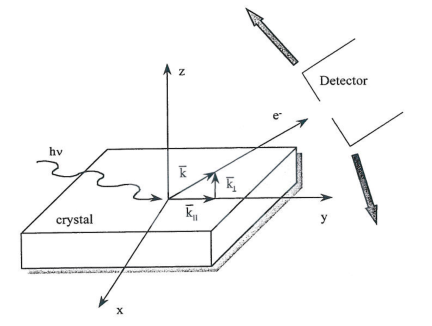
\includegraphics[scale=4]{figures/05_01.png}
	\caption{Schematics of the experimental set-up in an angle resolved UPS experiment.}
	\label{fig:arups}
	\end{center}
\end{figure}

A typical UPS spectrum of a transition metal is shown in \autoref{fig:cuups}. Here the d-band finger print can be found just below the Fermi level. It is also seen how the intensity increases towards low kinetic energy due to loss mechanisms. It is obvious that UPS cannot be used for identification of which elements that are present at the surface, since all metals (except for the rare earths) only exhibit broad and featureless structures in this region. 

\begin{figure}[h!]
	\begin{center}
	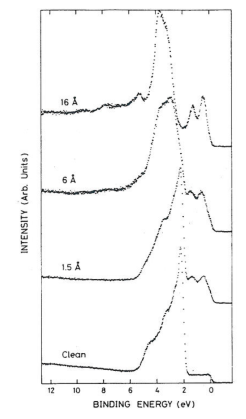
\includegraphics[scale=4]{figures/05_02.png}
	\caption{A UPS spectrum of clean Cu(100) with increasing amounts of samarium deposited. The photon energy was $h\nu=\SI{60}{\electronvolt}$. The sp-band of copper is observed just below the Fermi level, whereas the d-band is located at \SIrange{2}{4}{\electronvolt} binding energy. Taken from \cite{Andersen}.}
	\label{fig:cuups}
	\end{center}
\end{figure}

\section{The Electronic Structure}
\subsection{The Band Structure}
UPS and in particular ARUPS have been used to map out the band structure of solid materials. Here the outer electrons of the atoms react with each other forming a band structure with dispersion dependent on the momentum vector $\vec{k}$. \autoref{fig:bandstructure} shows the band structure for a simple free electron metal i.e. $E(k)=(\hbar k)^2/(2m)$. The photoemission process have to conserve both energy and momentum. Since the photon does not carry sufficient momentum to account for the momentum carried away by the photoelectron emitted the crystal must take care of the recoil. This is illustrated in the reduced zone where the electron takes up a reciprocal lattice vector and the process can be depicted as a direct transition in the reduced zone.

\begin{figure}[h!]
	\begin{center}
	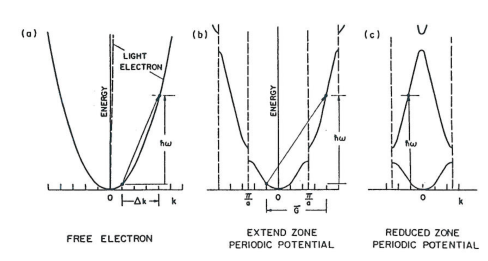
\includegraphics[scale=4]{figures/05_03.png}
	\caption{Sketch of the band structure of a free electron metal. Note the small momentum the photon carries compared to the electron. The transition can therefore only take place in the reduced zone where the lattice take up the recoil.}
	\label{fig:bandstructure}
	\end{center}
\end{figure}

By utilising the angle resolved method it is possible to map out the detailed band structure of a solid and in particular the structure at the surface region. An example is shown in \autoref{fig:cuarups} where the ARUPS spectra of Cu(111) are shown as a function of angle into the analyser using $h\nu=\SI{11.6}{\electronvolt}$.  The kinetic energy of the emitted  photoelectrons is given by

\begin{equation}
E_{kin}=h\nu-E_B-e\Phi
\end{equation}

\noindent where $E_B$ is the binding energy of the electron relative to the Fermi level, and $\Phi$ is the work function of the analyser.

\begin{equation}
E_{kin}=\frac{(\hbar k)^2}{2m}
\end{equation}

\noindent leading to 

\begin{equation}
k_\parallel=\sqrt{\frac{2mE_{kin}}{\hbar}}\sin \theta
\end{equation}

\noindent where $k_\parallel$  is the component of the momentum parallel to the surface.

\begin{figure}[h!]
	\begin{center}
	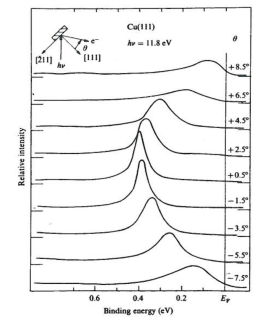
\includegraphics[scale=4]{figures/05_04.png}
	\caption{The ARUPS of Cu(111) as a function of the angle $\theta$ from the surface normal.}
	\label{fig:cuarups}
	\end{center}
\end{figure}

The momentum orthogonal to the surface $k_{\perp}$ is not conserved due to the work done by leaving the potential barrier at the surface (the work function of the crystal). By determining binding energy and $k_\parallel$ it is possible to map out the band structure around the $\Gamma$ point for Cu(111) as illustrated in Figure 5.5. The shown example is rather atypical since the shown band is a surface state lying in a bandgap. Usually there will be several bands overlapping and the gray zone indicated in \autoref{fig:cubandstructure} illustrates such  filled states in Cu(111), which in other directions will naturally cross the Fermi level since copper is known to be a metal. For a more detailed description of the band structure and how to measure it  we shall refer to \cite{Neddermeyer, Kevan}.

\begin{figure}[h!]
	\begin{center}
	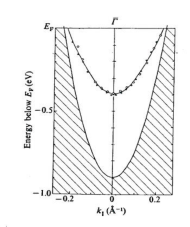
\includegraphics[scale=4]{figures/05_05.png}
	\caption{The band structure of the surface state in Cu(111) around the $\Gamma$ point. The gray zone illustrates the occupied bulk states.}
	\label{fig:cubandstructure}
	\end{center}
\end{figure}

Actually the experiment shown in \autoref{fig:cubandstructure} is a very simple example. In reality the measurement of such photoelectrons is a three step process  \cite{Berglund} where, firstly, the electron is excited from an initial band up into an empty band, secondly it have to be transported to the surface. In that process it may be diffracted as we shall see later and then  finally be detected. Thus diffraction phenomena may also have to be taken into account considering the details of such experiments.

\subsection{The Electronic Structure of Adsorbates}
When a molecule like CO (the test molecule of surface science) approaches a surface the electronic states will in general be broadened and lowered due to the interaction with the metal electrons. Thus, although the states are quite well defined in the gas phase they will now be rather broad as seen below in \autoref{fig:coups}. This figure shows the UPS spectra for gas phase CO and CO adsorbed on a number of transition metals like Ir, Ru, Pd, Pt, and Ni. The three highest occupied molecular levels of CO are easily identified in the gas phase spectrum, however, when CO chemisorbs the only feature which can be identified is due to the interaction with the valence electrons.  The contribution from the d-band is  in these late transition metals dominating the spectrum just below the Fermi level.

\begin{figure}[h!]
	\begin{center}
	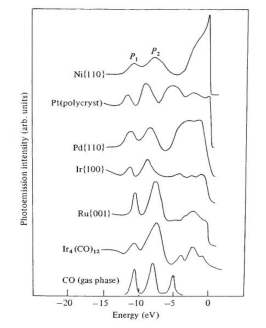
\includegraphics[scale=4]{figures/05_06.png}
	\caption{UPS of CO in the gas phase as well as CO adsorbed on a number of transition metals. Taken from Gustafson and Plummer \cite{Gustafson}.}
	\label{fig:coups}
	\end{center}
\end{figure}

Similar spectra can be observed for other adsorbates. Again it is seen that this cannot be used to identify adsorbates but solely to understand the bonding of already well defined systems. In this manner it was possible to understand the bonding geometry of for instance CO and also how molecules interact with each other as a function of coverage. Initially there was much dispute concerning the orientation of a chemisorbed molecule on a metal surface. Now it is well known that the molecule is bonded through the carbon in the "Blyholder  model"  and is standing orthogonal on the surface, at least in the low coverage regime. In the following we shall briefly demonstrate how such information can be obtained by using ARUPS and polarized light. The probability for photoelectron emission in second order time-dependent perturbation theory is given by

\begin{equation}
P_{if}=|<\Psi_{i}|{\bf H}_{int}|\Psi_f>|^2
\end{equation}

$\Psi_i$ and $\Psi_f$ are the electronic wave functions for the initial and final states and   ${\bf H}_{int}$ is the interaction Hamiltonian given by
 
\begin{equation}
{\bf H}_{int}\propto \vec{A}\cdot \vec{P}
\end{equation}
 
\noindent where $\vec{A}$ is the vector potential set up by the photon and $\vec{P}$ is the momentum operator

\begin{equation}
\vec{P}=\hbar \vec{\nabla}=\hbar \left(\frac{\partial}{\partial x}, \frac{\partial}{\partial y}, \frac{\partial}{\partial z}\right)
\end{equation}

Now lets assume that the CO molecule is adsorbed on top of a Ni atom on a Ni(100) surface which contains a mirror plane. Then the matrix element $<\Psi_i|{\bf H}_{int}|\Psi_f>$ must be invariant to such a symmetry operation, i.e. the matrix element must be even to the operation or zero. The experiment is shown schematically in \autoref{fig:arupspol}

\begin{figure}[h!]
	\begin{center}
	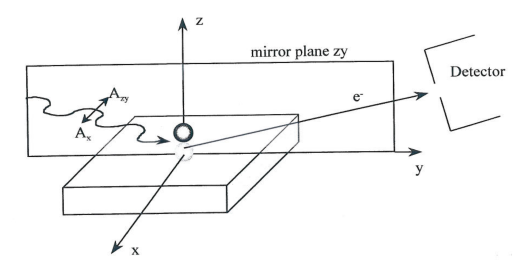
\includegraphics[scale=3.5]{figures/05_07.png}
	\caption{ An ARUPS experiment using polarised light on a surface containing a mirror plane in the $zy$-plane.}
	\label{fig:arupspol}
	\end{center}
\end{figure}

Assume the mirror plane is lying in the $zy$-plane and the detector is located in this plane as well, then the final state  $\Psi_f$ must be even with respect to the symmetry operation or zero, i.e. no signal in the detector. We then have two possibilities for the incoming light. It can either be s-polarised i.e. the vector potential only has components parallel to the surface or p-polarised where it has components orthogonal to the surface. It is then easily seen that if we consider s-polarised light the product $\vec{A}\cdot \vec{P}$ will give a product that will be odd with respect to the reflection in the $zy$-plane since $\Psi_f$ should be even if anything should be detected. Thus $\Psi_i$ must be odd in order for the matrix element to be even. Thus it is only possible to excite molecular orbitals that are odd with s-polarised light in the given configuration. This is clearly illustrated in \autoref{fig:arupsspol} where it is seen that for a certain configuration the even $4\sigma$ is vanishing in the spectrum, while the odd $1\pi$ still is observed.

\begin{figure}[h!]
	\begin{center}
	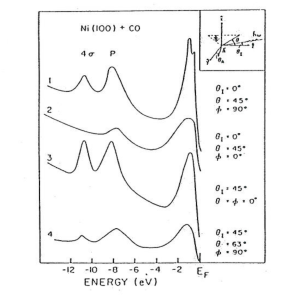
\includegraphics[scale=4.5]{figures/05_08.png}
	\caption{The result of an ARUPS experiment where the use of s-polarised light suppresses the signal from the even $4\sigma$ while the odd $1\pi$ can still be observed. For other combinations both orbitals are observed.}
	\label{fig:arupsspol}
	\end{center}
\end{figure}

The symmetry of the various orbitals of CO are reproduced in \autoref{fig:orbitals}. By playing around with the geometry like this it is possible to describe the geometry of the chemisorbed CO molecule. It has been show that the molecules tend to tilt when the coverage gets very high in order to accommodate the last CO molecules.

\begin{figure}[h!]
	\begin{center}
	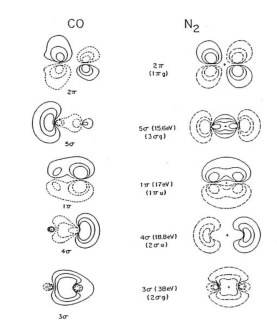
\includegraphics[scale=4.5]{figures/05_09.png}
	\caption{Sketches of the molecular orbital for CO and \ce{N2}. Notice that the $\sigma$ orbitals are even with respect to the molecular axis while the $\pi$ orbitals are odd.}
	\label{fig:orbitals}
	\end{center}
\end{figure}

The method has played a very big role in the infancy of surface science, e.g. to reveal the orientation and bonding geometry of molecules on the surface.